\documentclass[11pt]{article}

\usepackage{fullpage}
\usepackage{amsmath}
\usepackage{fancyhdr}
% \renewcommand{\familydefault}{\rmdefault}
% \usepackage{paralist}
%\usepackage{times,graphicx,epstopdf,,amsfonts,amsthm,amsmath,xspace}
%\usepackage[left=.75in,top=.75in,right=.75in,bottom=.75in]{geometry}
% \usepackage{hyperref}
% \usepackage[ruled,vlined,linesnumbered]{algorithm2e}
\usepackage{enumitem}
\usepackage{amsmath,amsthm,amssymb}
\usepackage{comment}
\usepackage{multicol}
\usepackage{float}
\restylefloat{table}
% \usepackage[
% singlelinecheck=false % <-- important
% ]{caption}
% \usepackage{blindtext}
% \usepackage{xspace}
% \usepackage{listings}
% \newtheoremstyle{case}{}{}{}{}{}{:}{ }{}
% \theoremstyle{case}
% \newtheorem{case}{Case}

% \newtheorem*{theorem*}{Theorem}
% \newtheorem{theorem}{Theorem}

% \newcommand{\set}[3]{{\{{#1}\}}}

\pdfpagewidth 8.5in
\pdfpageheight 11in 

%\pagestyle{fancy}
\renewcommand{\qedsymbol}{$\blacksquare$}
\oddsidemargin 0in
\evensidemargin 0in

\newtheorem*{claim}{Claim}
\newtheorem{definition}{Definition}
\newtheorem{lemma}{Lemma}
\newtheorem{observation}{Observation}
\newtheorem{question}{Question}
\newtheorem{problem}{Problem}
\usepackage{graphicx}
%
\newcommand\independent{\protect\mathpalette{\protect\independenT}{\perp}}
\def\independenT#1#2{\mathrel{\rlap{$#1#2$}\mkern2mu{#1#2}}}

\makeatletter
\renewcommand*\env@matrix[1][*\c@MaxMatrixCols c]{%
  \hskip -\arraycolsep
  \let\@ifnextchar\new@ifnextchar
  \array{#1}}
\makeatother

%----------------------------------------------------------------------------------------------
% Pset Name, Date, Author
%----------------------------------------------------------------------------------------------
\title{ CS 506 \\ Consumer ABS}
\date{23 November 2020}
\author{James Bishop }
\begin{document}

\maketitle

\section*{How has the current interest rate environment impacted consumer ABS pricing?}
In the years following the Great Financial Crisis, dovish Federal Reserve policies deflated the front of the yield curve dramatically in order to offset the massive economic impact of what we now know was a credit bubble \ref{YieldCurve}. In the near term, consumers strayed away from debt as best they could, but the main outcome of the GFC was not a change in consumer sentiment but rather changes in banking regulation and operations along with the longest bull run to date in equity markets. \begin{figure}[h]
    \centering
    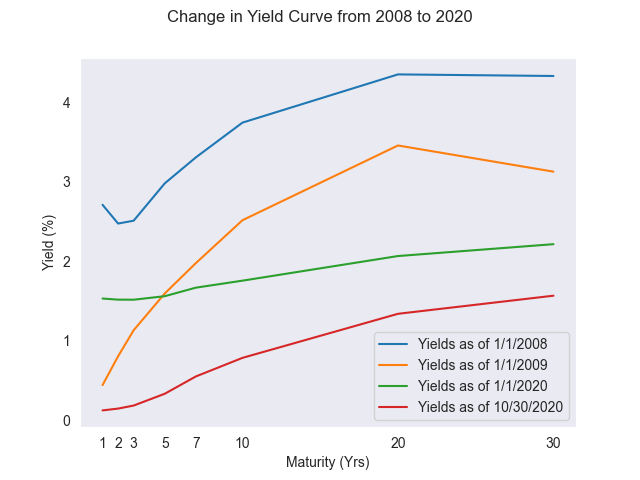
\includegraphics[scale=0.5]{YieldCurve}
    \caption{Your caption}
    \label{YieldCurve}
\end{figure}

In the months before the COVID-19 pandemic, the yield curve had flattened out with the front end rising and back end falling. 


\section*{How has consumer ABS pricing evolved as US consumer debt grows over \$14.3 trillion?}


\section*{What does the composition of the average auto, credit, or student-loan backed ABS look like and does the riskiness of the security seem properly priced?}







\end{document}
